\documentclass[10pt]{beamer}
\usepackage{verbatim}
\usepackage{graphicx}
\title{Getting Real -- The Secrets of 37signals}
\author{George Rogers}
\begin{document}
\begin{frame}
  \titlepage
  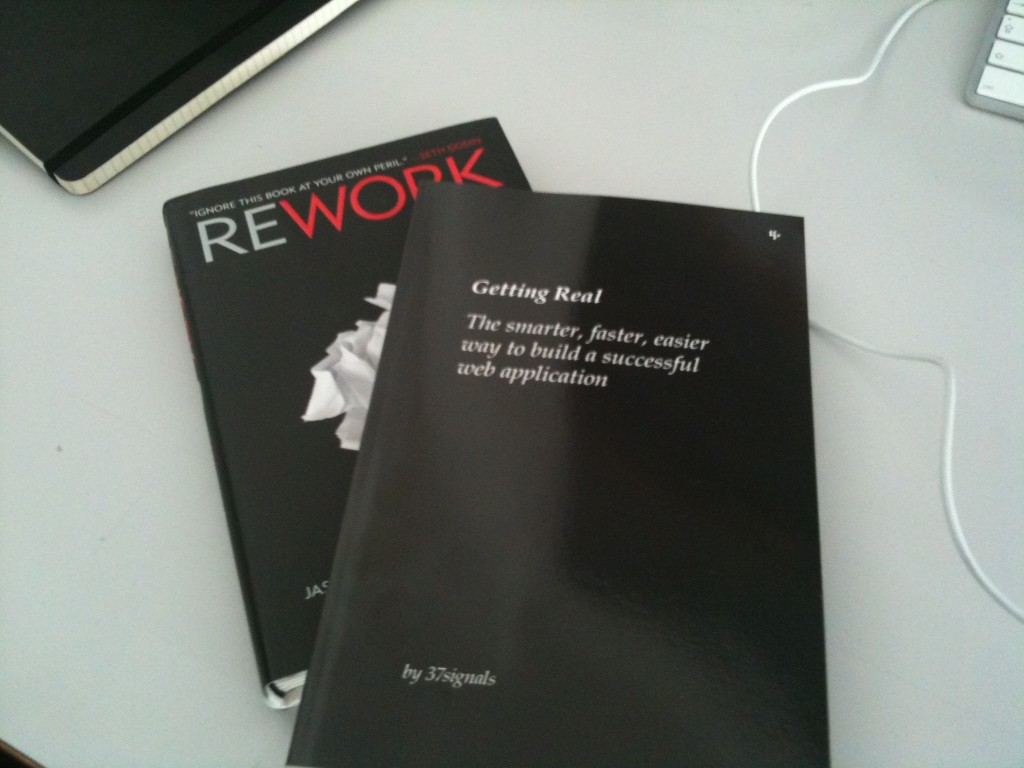
\includegraphics[width=2in]{books}
\end{frame}
\begin{frame}
  \frametitle{What You Will Learn}
  \pause
  \begin{itemize}
  \item About 37signals.
  \pause
  \item Feature Selection
    \begin{itemize}
    \item Less Is More
    \item Half NOT Half Hearted
    \item Forget Feature Requests
    \end{itemize}
  \pause
  \item Process
    \begin{itemize}
    \item Race to running software
    \item Iterate
    \item Done!
    \end{itemize}
  \pause
  \item Code
    \begin{itemize}
    \item Less Software
    \item Optimize For Programmer Happiness
    \item Refactor, Refactor, Refactor!
    \end{itemize}
  \end{itemize}
\end{frame}
\begin{frame}
  \frametitle{WHY?}
  \pause
  \begin{itemize}
    \item 37signals is a profitable company; that produces products:
      on time, and on budget
    \pause
    \item 37signals makes some of the most useful web applications with
      a small team.
    \pause
    \item They made the best web framework: Ruby On Rails.
  \end{itemize}
\end{frame}
\begin{frame}
  \frametitle{About 37signals}
  Products
  \pause
  \begin{itemize}
  \item Basecamp -- A Project Manager and Their First Product.
   \pause
  \item Highrise -- A Contact Manager
  \pause
  \item Campfire -- A Corporate Chat Service
  \end{itemize}
\end{frame}
\begin{frame}
  \frametitle{Feature Selection}
  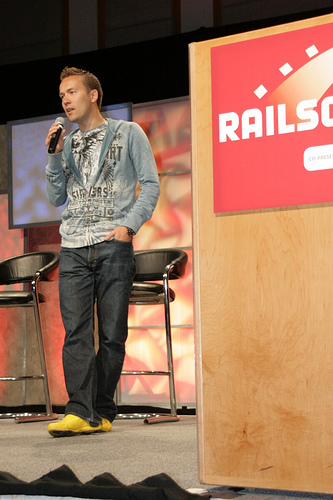
\includegraphics[height=2in]{dhh-railsconf}
\end{frame}
\begin{frame}
  \frametitle{Less Is More}
  \pause
  \begin{itemize}
  \item Less Features $=$ Easier To Use
  \pause
  \item Some Features ARE Misfeatures
  \pause
  \item Less Features $=$ Less Work
  \end{itemize}
\end{frame}
\begin{frame}
  \frametitle{Half NOT Half Hearted}
  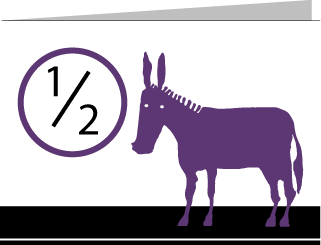
\includegraphics[height=1in]{halfass}
  \pause
  \begin{itemize}
  \item It is better to have HALF of the ideal product,
    than have a slipshod implementation of the whole shebang.
    \pause
  \item Have you ever used something where the features get in the way.
    Those features are called Misfeatures.
    \pause
  \item Your product will be more focused.
  \end{itemize}
\end{frame}
\begin{frame}
  \frametitle{How to process feature requests}
  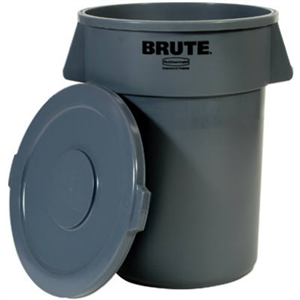
\includegraphics[height=1in]{trashcan}
  \pause

  \begin{enumerate}
    \item Receive it
      \pause
    \item Read it
      \pause
    \item Forget it
      \pause
  \end{enumerate}
  The good feature requests: you will remember them because you receive them very often.
\end{frame}
\begin{frame}
  \frametitle{Process}
  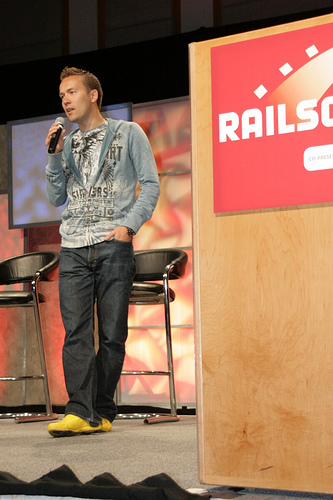
\includegraphics[height=2in]{dhh-railsconf}
\end{frame}
\begin{frame}
  \frametitle{Race To Running Software}
  \pause
  \begin{itemize}
  \item Prototype DON'T plan
    \pause
  \item Prototypes will help
    \begin{itemize}
      \pause
    \item Increase agreement
      \pause
    \item Improve the quality of your product
      \pause
    \item Select the right features
    \end{itemize}
  \end{itemize}
\end{frame}
\begin{frame}
  \frametitle{Iterate}
  \pause
  \begin{itemize}
  \item Iteration allows you to make decisions by trying things out
    \pause
  \item If they don't work just throw them out
    \pause
  \item Reduces cruft by figuring out whats really necessary.
  \end{itemize}
\end{frame}
\begin{frame}
  \frametitle{Done!}
  \pause
  \begin{itemize}
    \item Reduce scope to meet deadline -- not quality or cost
    \pause
    \item Sacrifice Features -- Not Quality
    \pause
    \item Don't throw programmers at the problem
  \end{itemize}
\end{frame}
\begin{frame}
  \frametitle{Code}
  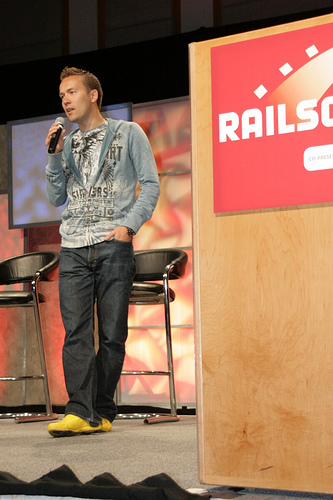
\includegraphics[height=2in]{dhh-railsconf}
\end{frame}
\begin{frame}
  \frametitle{Less Software}
  \begin{itemize}
  \item Less Software $=$ Better Software
    \pause
  \item Less Software Costs Less
    \pause
  \item Less Software $=$ Less Bugs
  \end{itemize}
\end{frame}
\begin{frame}
  \frametitle{Optimize for Programmer Happiness}
  \pause
  \begin{itemize}
    \item Programmers are people
    \pause
    \item People like doing more work with less effort
    \pause
    \item Select programming languages that make programmers happy
  \end{itemize}
\end{frame}
\begin{frame}
  \frametitle{How?}
  Print to the console the numbers 0 through 9.
  \begin{block}{Ruby}
    \verbatiminput{hello.rb}
  \end{block}
  \begin{block}{Java}
    \verbatiminput{Hello.java}
  \end{block}
\end{frame}
\begin{frame}
  \frametitle{Refactor, Refactor, Refactor!}
  \begin{itemize}
    \item Refactoring is the process of cleaning up code
    \pause
    \item Code can be written in a way that is messy
    \pause
    \item If you don't clean it up it will get messier and messier
  \end{itemize}
\end{frame}
\begin{frame}
  \frametitle{What You Learned}
  \pause
  \begin{itemize}
  \item About 37signals.
  \pause
  \item Feature Selection
    \begin{itemize}
    \item Less Is More
    \item Half NOT Half Hearted
    \item Forget Feature Requests
    \end{itemize}
  \pause
  \item Process
    \begin{itemize}
    \item Race to running software
    \item Iterate
    \item Done!
    \end{itemize}
  \pause
  \item Code
    \begin{itemize}
    \item Less Software
    \item Optimize For Programmer Happiness
    \item Refactor, Refactor, Refactor!
    \end{itemize}
  \end{itemize}
\end{frame}
\end{document}
